\chapter{Content Chapter}
\label{sec:Content Chapter}


\section{Research Methodology}
\label{sec:Research Methodology}

 For this project, a design research methodology will be utilized to solve the problem. Since this project requires a design research methodology to be completed, there is a structure that can be followed. The initial phase that needs to be completed is a design requirement phase. In this section it required to determine:

\begin{itemize}
    \item Stakeholders;
    \item Design independent parameters (DIP);
    \item Boundary between wider system of interest and narrower system of interest;
    \item Functional Requirement;
    \item Non-functional Requirements;
    \item Technical performance measures (TPM);
\end{itemize}

of the system. It is essential to remain neutral in this section.


The second phase that needs to be completed is the concept development phase. In this section, concepts are developed and described to meet all the requirement in the design requirement phase. These concepts are evaluated before the best concept or combination of concepts is selected. The selected concept(s) is refined further, before a final evaluation is performed.


The last 2 sections of this methodology is the detail design and analysis phase; which is then followed with the evaluation phase. The detail design and analysis phase requires the researcher to utilize the refined concept from the preceding section and create a detail design of the concept. This process does require an iterative process to create the final design. A drawing pack is required at the end of this phase that will be evaluated. The evaluation phase consists of evaluating the developed product. This includes building the product, before it can be tested. Based on the test results of the product, an evaluation can be performed.


\section{Workplan}

This section of the proposal covers the planned workplan that will be conducted for this project. As established in the prior \textit{section} \textit{\ref{sec:Research Methodology}}, this project will follow a design research methodology. Therefore, it can be assumed that the project will require these following activities:

\subsection{Literature Review}

Study the literature of laparoscopic surgery to gain an understanding of the conditions that a laparoscope will experience. Consequently, there will be required to study literature that will inform what attributes the developed laparoscope should satisfy, to be used for testing purposes on future projects.

\subsection{Component Review}

A detailed investigation was conducted to create a list of possible hardware components, which can be used to integrate within the developed product. The hardware components that were investigated are:

\begin{itemize}
    \item Single board computers.
    \item Camera modules.
    \item Illumination modules.
    \item Display modules.
\end{itemize}

Except for the camera modules, only local supplier stock were investigated for this project, since they have adequate products available. Except for the DF Robot endoscope, mentioned in \textit{subsection} \textit{\ref{sec:Camera Module}}, no other products were found to meet the physical demands in South African suppliers for the camera modules. Henceforth, the reason why international companies were investigated for possible solutions for the camera module of the project. 

\subsection{Compile Design Requirements for Laparoscope}

As mentioned in \textit{section \ref{sec:Research Methodology}}, there are a list of requirements that needs to be determined. These requirements are all listed in the tables below, as well as shown in the diagrams below. The stakeholder analysis is shown in \textit{table \ref{tab:stakeholders}} below:

\begin{longtable}{|p{0.10\textwidth}|p{0.10\textwidth}|p{0.121\textwidth}|p{0.18\textwidth}|p{0.12\textwidth}|p{0.18\textwidth}|}

    \caption{Stakeholder Analysis}              % ← Moved to top
    \label{tab:stakeholders}\\
% ---- FIRST PAGE HEADER ----
\hline
\textbf{Stake-holder ID} & 
\textbf{Stake-holder} & 
\textbf{Class-ification} & 
\textbf{Description} & 
\textbf{Life Cycle Stages} & 
\textbf{Key Interest/Needs} \\
\hline
\endfirsthead

% ---- SUBSEQUENT PAGE HEADER ----
\hline
\textbf{Stake-holder ID} & 
\textbf{Stake-holder} & 
\textbf{Class-ification} & 
\textbf{Description} & 
\textbf{Life Cycle Stages} & 
\textbf{Key Interest/Needs} \\
\hline
\endhead

% ---- FOOTER ALL PAGES EXCEPT LAST ----
\hline
\multicolumn{6}{r|}{\textit{Continued on next page...}} \\
\hline
\endfoot

% ---- LAST PAGE FOOTER ----
\endlastfoot

% ---- SH_01 ----
SH\_01 & 
Dr Diayar & 
Indirect & 
The doctor that recommend the development of the system & 
Concept & 
The functional development of the system \\
\hline

% ---- SH_02 ----
SH\_02 & 
Prof Schreve & 
Secon-dary & 
Supervisor of the project & 
All stages & 
The functional development of the system, and the engineering 
design methodology followed to develop the system \\
\hline

% ---- SH_03 ----
SH\_03 & 
Medical trainee & 
Primary & 
The personal that will use the developed system to improve 
their surgical abilities & 
Opera-tion & 
The low-cost production of the system and the easy operations 
of the system \\
\hline

% ---- SH_04 ----
SH\_04 & 
Hard-ware supp-liers & 
Secon-dary & 
The suppliers of the hardware components for the system & 
Design, Installation & 
Technical specifications of the hardware components \\
\hline

% ---- SH_05 ----
SH\_05 & 
Struc-tural manu-factur-ers & 
Secon-dary & 
Personnel responsible for the construction of structural 
components of the system & 
Design, Installation & 
Technical specifications of the structural components \\
\hline

% ---- SH_06 ----
SH\_06 & 
Stellen-bosch Univer-sity & 
Secon-dary & 
Main financial supplier and main management team of 
the project & 
All stages & 
The cost of the project, academic procedures followed 
and safe operations during all stages of the project \\
\hline

% ---- SH_07 ----
SH\_07 & 
Future resear-chers & 
Primary & 
Future personal that will use the developed system or select 
components of the system to perform further researchers & 
Mainte-nance, Operation & 
The technical conditions of the developed system, the 
technical conditions of systems hardware components \\
\hline

% ---- SH_08 ----
SH\_08 & 
Con-struc-tion and maintenance staff & 
Secon-dary & 
Personnel responsible for the construction and maintenance 
for the entire system & 
Installa-tion, Maintenance & 
System design and building procedures, systems maintenance 
procedures \\
\hline

% ---- SH_09 ----
SH\_09 & 
Design team & 
Secon-dary & 
Personnel responsible for the design of the entire system & 
Design & 
System requirement and hardware physical properties \\
\hline

% ---- SH_10 ----
SH\_10 & 
Soft-ware team & 
Secon-dary & 
Personnel for the software component of the entire system & 
Design, Installation & 
System requirements and hardware software capabilities \\
\hline

% ---- SH_11 ----
SH\_11 & 
Poten-tial student attendees & 
Primary & 
Potential students that will use the system to perform 
surgical procedures & 
Opera-tion & 
Easy operations and usability of the system \\
\hline

\end{longtable}


The DIP requirements for the laparoscope can be seen in \textit{table \ref{tab:DIP}} below. Additionally, how the DIPs interface from the narrower system of interest (NSOI) with the wider system of interest (WSOI) and environment can be seen in \textit{figure \ref{fig:System Boundary}} below:

\begin{longtable}{|p{0.12\textwidth}|p{0.35\textwidth}|p{0.15\textwidth}|p{0.23\textwidth}|}

\caption{Design Independent Parameters}        
\label{tab:DIP} \\                             

% ---- FIRST PAGE HEADER ----
\hline
\textbf{DIP\_ID} & 
\textbf{Design Independent Parameter Description} & 
\textbf{Value / Range} & 
\textbf{Reference} \\
\hline
\endfirsthead

% ---- SUBSEQUENT PAGE HEADER ----
\hline
\textbf{DIP\_ID} & 
\textbf{Design Independent Parameter Description} & 
\textbf{Value / Range} & 
\textbf{Reference} \\
\hline
\endhead

% ---- FOOTER ALL PAGES EXCEPT LAST ----
\hline
\multicolumn{4}{r|}{\textit{Continued on next page...}} \\
\hline
\endfoot

% ---- LAST PAGE FOOTER ----
\endlastfoot

% ---- DIP_01 ----
DIP\_01 & 
Laparoscope maximum \mbox{diameter} & 
$\varnothing$ < 10 mm & 
Supervisor \\
\hline

% ---- DIP_02 ----
DIP\_02 & 
Grid electricity availability & 
230 V, 15 Ampere at 50 Hz & 
worldstandards.eu \\
\hline

% ---- DIP_03 ----
DIP\_03 & 
Ambient operating temperatures range (Stellenbosch) & 
2 C$^{\circ}$ - 42 C$^{\circ}$ & 
weather-and-climate.com \\
\hline

% ---- DIP_04 ----
DIP\_04 & 
Laparoscopes total \mbox{building cost} & 
R 6000.00 & 
Stemlearn (2026) \\
\hline

% ---- DIP_05 ----
DIP\_05 & 
Laparoscope illuminance produced & 
40 000 LUX - 160 000 LUX & 
IEC 60601-2-41:2021 \\
\hline

% ---- DIP_06 ----
DIP\_06 & 
Relative maximum humidity in operating rooms & 
< 81\% & 
weather-and-climate.com \\
\hline

% ---- DIP_07 ----
DIP\_07 & 
Maximum deviation of specified viewing angle & 
10$^{\circ}$ & 
ISO 8600-1:2025 \\
\hline

% ---- DIP_08 ----
DIP\_08 & 
Frequency of real-time \mbox{digital} images updates & 
30 Hz - 60 Hz & 
\citep{KSE-TR} \\
\hline

\end{longtable}

\begin{figure}[H]
    \centering
    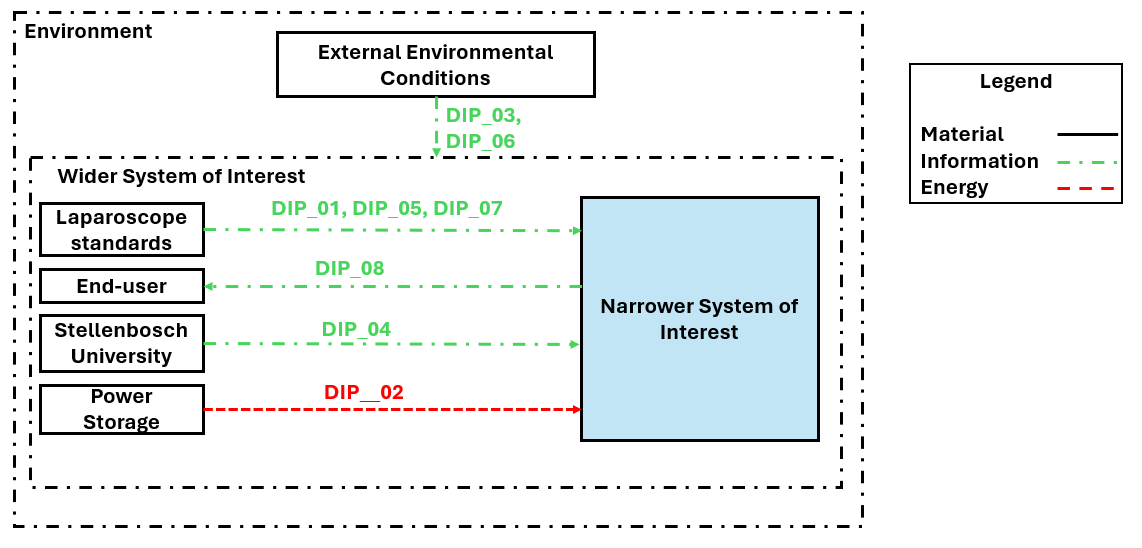
\includegraphics[height=6cm]{figs/System Boundary.png}
    \caption{System Boundary}
    \label{fig:System Boundary}
\end{figure}

Below in \textit{table \ref{tab:FR}} is the functional requirements for the laparoscope. Consequently, the \textit{table \ref{tab:NFR}} contains the non-functional requirements.

\begin{longtable}{|p{0.10\textwidth}|p{0.55\textwidth}|p{0.25\textwidth}|}

\caption{Functional Requirements}
\label{tab:FR} \\

% ---- FIRST PAGE HEADER ----
\hline
\textbf{FR\_ID} & 
\textbf{Functional Requirement Description} & 
\textbf{Primary/Derived} \\
\hline
\endfirsthead

% ---- SUBSEQUENT PAGE HEADER ----
\hline
\textbf{FR\_ID} & 
\textbf{Functional Requirement Description} & 
\textbf{Primary/Derived} \\
\hline
\endhead

% ---- FOOTER ALL PAGES EXCEPT LAST ----
\hline
\multicolumn{3}{r|}{\textit{Continued on next page...}} \\
\hline
\endfoot

% ---- LAST PAGE FOOTER ----
\endlastfoot

% ---- DATA ROWS ----
FR\_1 & User interface & Primary \\
\hline

FR\_2 & System processor & Primary \\
\hline

FR\_3 & Power supply & Primary \\
\hline

FR\_4 & Operate Camera Module & Primary \\
\hline

FR\_4.1 & Specify camera settings & Derived \\
\hline

FR\_4.2 & Specify light intensity & Derived \\
\hline

FR\_4.3 & Capture digital image & Derived \\
\hline

FR\_5.0 & Display real-time images & Primary \\
\hline

FR\_6.0 & Store system data & Primary \\
\hline

\end{longtable}

\begin{longtable}{|p{0.12\textwidth}|p{0.25\textwidth}|p{0.55\textwidth}|}

\caption{Non-Functional Requirements}
\label{tab:NFR} \\

% ---- FIRST PAGE HEADER ----
\hline
\textbf{NFR\_ID} & 
\textbf{Non-Functional Requirement} & 
\textbf{Description}       \\                    
\hline
\endfirsthead

% ---- SUBSEQUENT PAGE HEADER ----
\hline
\textbf{NFR\_ID} & 
\textbf{Non-Functional Requirement} & 
\textbf{Description} \\                         % ← Please provide last column heading
\hline
\endhead

% ---- FOOTER ALL PAGES EXCEPT LAST ----
\hline
\multicolumn{3}{r|}{\textit{Continued on next page...}} \\
\hline
\endfoot

% ---- LAST PAGE FOOTER ----
\endlastfoot

% ---- NFR_01 ----
NFR\_01 & 
Relevant \mbox{compliance} & 
The design of the system should meet the relevant 
prescribed standard for this project, to ensure that 
the laparoscope meets all physical capabilities and 
functionality of a real laparoscope     \\                            
\hline

% ---- NFR_02 ----
NFR\_02 & 
Documentation & 
The design, implementation, construction, maintenance 
and testing procedures for the system should be 
thoroughly documented       \\                           
\hline

% ---- NFR_03 ----
NFR\_03 & 
Availability & 
The components for this project should be available 
to purchase if a component breaks or should be 
replaced \\
\hline

% ---- NFR_04 ----
NFR\_04 & 
Adjustable & 
The system design should be developed that distinct 
features can be changed without creating large 
external costs \\
\hline

% ---- NFR_05 ----
NFR\_05 & 
Usability & 
System should be easy to operate for limited-training 
users \\
\hline

\end{longtable}

The TPMs can be seen in the \textit{table \ref{tab:FR-TPM}} below, based on the values in \textit{table \ref{tab:FR}}. The reasoning behind all the TPM target values can be found below the table.

\begin{longtable}{|p{0.1\textwidth}|p{0.15\textwidth}|p{0.11\textwidth}|p{0.25\textwidth}|p{0.20\textwidth}|}

\caption{Functional Requirements and Technical Performance Measures}
\label{tab:FR-TPM} \\

% ---- FIRST PAGE HEADER ----
\hline
\textbf{FR\_ID} & 
\textbf{Function} & 
\textbf{TPM\_ID} & 
\textbf{TPM Description} & 
\textbf{TPM Target Value(s)} \\
\hline
\endfirsthead

% ---- SUBSEQUENT PAGE HEADER ----
\hline
\textbf{FR\_ID} & 
\textbf{Function} & 
\textbf{TPM\_ID} & 
\textbf{TPM Description} & 
\textbf{TPM Target Value(s)} \\
\hline
\endhead

% ---- FOOTER ALL PAGES EXCEPT LAST ----
\hline
\multicolumn{5}{r|}{\textit{Continued on next page...}} \\
\hline
\endfoot

% ---- LAST PAGE FOOTER ----
\endlastfoot

% ---- FR_1.0 - User Interface (2 TPMs) ----
\multirow{2}{*}{FR\_1.0} & 
\parbox[t]{\linewidth}{User \mbox{interface}} & 
TPM\_01 & 
Minimum user interface input(s) & 
$\geq$ 1 input \\
\cline{3-5}

& & 
TPM\_02 & 
Minimum user interface signal(s) & 
$\geq$ 1 signal light \\
\hline

% ---- FR_2.0 - System Processor (1 TPM) ----
FR\_2.0 & 
System \mbox{processor} & 
TPM\_03 & 
Minimum GPIO pins & 
$\geq$ 1 GPIO Pin \\
\hline

% ---- FR_3.0 - Power Supply (2 TPMs) ----
\multirow{2}{*}{FR\_3.0} & 
\parbox[t]{\linewidth}{Power \mbox{supply}} & 
TPM\_04 & 
System start up cycle duration & 
$\leq$ 2 s \\
\cline{3-5}

& & 
TPM\_05 & 
Total duration of power supply required & 
$\geq$ 6.7 hours \\
\hline

% ---- FR_4.0 - Operate Camera Module (3 TPMs) ----
\multirow{3}{*}{FR\_4.0} & 
\parbox[t]{\linewidth}{Operate camera module} & 
TPM\_06 & 
Amount of camera modules & 
1 camera modules \\
\cline{3-5}

& & 
TPM\_07 & 
Working length of the system & 
300 mm \\
\cline{3-5}

& & 
TPM\_08 & 
Viewing angle of camera module & 
30$^{\circ}$ \\
\hline

% ---- FR_4.1 - Configure Camera Properties (1 TPM) ----
FR\_4.1 & 
\makecell[l]{Configure \\camera \\properties} & 
TPM\_09 & 
Focus depth of the camera module & 
30 mm - 80 mm \\
\hline

% ---- FR_4.2 - Configure Light Intensity (2 TPMs) ----
\multirow{2}{*}{FR\_4.2} & 
\parbox[t]{\linewidth}{Configure light \mbox{intensity}} & 
TPM\_10 & 
Illumination of system & 
40 000 LUX - 160 000 LUX \\
\cline{3-5}

& & 
TPM\_11 & 
Maximum surface temperature & 
$\leq$ 41 $^{\circ}$C \\
\hline

% ---- FR_4.3 - Capture Digital Image (2 TPMs) ----
\multirow{2}{*}{FR\_4.3} & 
\parbox[t]{\linewidth}{Capture digital image} & 
TPM\_12 & 
Minimum field of view & 
$\geq$ 70$^{\circ}$ \\
\cline{3-5}

& & 
TPM\_13 & 
Minimum resolution & 
460 x 460 pixels \\
\hline

% ---- FR_5.0 - Display Real-Time Images (2 TPMs) ----
\multirow{2}{*}{FR\_5.0} & 
\parbox[t]{\linewidth}{Display real-time images} & 
TPM\_14 & 
Minimum resolution of display & 
460 x 460 pixels \\
\cline{3-5}

& & 
TPM\_15 & 
Maximum latency & 
0.5 s \\
\hline

% ---- FR_6.0 - Store System Data (1 TPM) ----
FR\_6.0 & 
Store system data & 
TPM\_16 & 
Storage capacity & 
68.56 GB \\
\hline

\end{longtable}

\begin{itemize}
     

    \item\textbf{TPM\_01:} The bare minimum for the laparoscope to function properly with user inputs is to at least install an on or off switch. It is the bare minimum required for this project.

    \item\textbf{TPM\_02:} For the operator to know the laparoscope is still functioning properly, without looking at the display screen or light module at the end of the laparoscope, there should be at least 1 signal light on the laparoscope to indicate that the system is receiving power.

    \item\textbf{TPM\_03:} To operate the signal lights the microcontroller or SBC will require GPIO pin to push current into the signal lights. Thus, the minimum required is the minimum of the laparoscope signal lights.

    \item\textbf{TPM\_04:} This is dependent on the component selected and the different interfaces selected between the different components. However, the desired start-up cycle duration should be less than 2 seconds.

    \item\textbf{TPM\_05:} The system should be able to power on for long durations of times. The total amount of time it should be powered on is the duration of a typical laparoscopic surgery. 

    \item\textbf{TPM\_06:} The system requires at least 1 laparoscopic camera. A second camera module can help the system achieve 3D visualization. Any additional cameras would be redundant for this project.

    \item\textbf{TPM\_07:} The system design should be similar to current laparoscopes. Current laparoscope designs has a working distance of 300 mm. The working distance is the distance of the rod that can be inserted into the patient's body.

    \item\textbf{TPM\_08:} Different laparoscope products have different viewing angles. Some has a viewing angle of 0°, while there are products that have a viewing angle of 90°. However, a common viewing angle is 30°, which is the value that will be pursued in this project.

    \item\textbf{TPM\_09:} The distance between the camera sensor of the laparoscope and the object that is being captured is the focus depth. 

    \item\textbf{TPM\_10:} The total illumination required per medical theatres.
    
    \item\textbf{TPM\_11:} The maximum temperature of the casing of the laparoscope tip, based on medical standards.

    \item\textbf{TPM\_12:} Smallest viewing angle applied to a laparoscopic commercial product is 70°,  while certain laparoscopes has a viewing angle larger than 70°.

    \item\textbf{TPM\_13:} The minimum resolution for the camera module is determined by the first determining the maximum visible seen at the smallest fov, and multiply that value with how many pixels a millimetre area should represent: Pixel = Focus depth\_(max)*sin(fov/2)*2*5 pixels/mm.

    \item\textbf{TPM\_14:} The minimum resolution of the display is the same as the minimum resolution of the camera.

    \item\textbf{TPM\_15:} This value is subject to change based on the different components used for the system. Therefore, it is important to minimize the latency of each component or interaction between different components. 0.5 s is just an absolute maximum latency that will be accepted.

    \item\textbf{TPM\_16:} If the minimum resolution an image is 460 x 460 with RGB colour format, then 1 image requires 634.8 KB. (PxP*24/8) If the frame rate is 30 fps and this continued for 60 minutes, then a total space of 68.5584 Gb is required.

\end{itemize}
\subsection{Generate Concept Design for Laparoscope}

For this project 3 concepts were generated, based on the principle that it utilized the DF Robot endoscope, which has the dimensions of Ø8~mm and a total length of 25~mm. This module was chosen, since it is the maximum minimum space required to fit all the necessary PCB and camera assembly to create an endoscope, that still fit within the Ø10~mm hole. Each concept is design to have a viewing angle of 30°.

The first concept, relies on bending the shaft that the endoscope camera is attached to. However, the total diameter of the laparoscope within the skin and muscle tissue of the patient should remain under the Ø10~mm limit. Since, the thickness of the muscle and tissue of patients are not all the same, the design has to be made for the worst case scenario, which is for an obese patient around 10 cm. \textit{Figure \ref{fig:Concept 1}} below illustrates how the design would look like:

\begin{figure}[H]
    \centering
    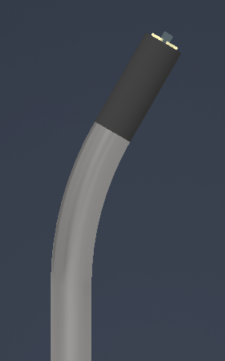
\includegraphics[height = 8 cm]{figs/Concept 1.png}
    \caption{Concept 1: Bent shaft design}
    \label{fig:Concept 1}
\end{figure}

The second concept, rely on that the lens assembly is tilted to 30° relative to the axial axis of the laparoscope. This concept, does require careful hardware consideration and positioning, however is a proven method in the industry. \textit{Figure \ref{fig:Concept 2}} illustrates this design:

\begin{figure}[H]
    \centering
    
\includegraphics[height = 8 cm]{figs/Concept 2.png}
    \caption{Concept 2: Tilted lens design}
    \label{fig:Concept 2}
\end{figure}

The last concept, relies on a pulley system, which allows the camera to be tilted at a desired angle by the practitioner, while the operation is being performed. This method relies on fine detail design, but can prove to be beneficial for future research purposes. The final concept is illustrated in \textit{figure \ref{fig:Concept 3}} below:

\begin{figure} [H]
    \centering
    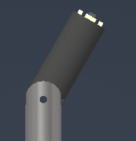
\includegraphics[height = 8 cm]{figs/Concept 3.png}
    \caption{Concept 3: Adjustable viewing angle design}
    \label{fig:Concept 3}
\end{figure}

All 3 concept mentioned above can be used for the project, since they meet all physical demands of the laparoscope. However, each concept has their defects. Concept 1 and 3, have both a defect when their camera is tilted at 30°. When the laparoscope is being rotated, there might be vital information that is missed in the direction of the laparoscopes axial axis, due to the camera lenses not being centred on the axis itself. It can also possibly cause damage to the patients, if the laparoscopes are being turned and accidentally being pushed into the patients internal organs.

Due to the reason stated above, the second concept is the preferred concept that will be further developed.

\subsection{Finalize Detail Design for Laparoscope}

Design and finalize the selected concept design of the laparoscope. This includes producing relevant calculations and analysis of the developed laparoscope and the full drawing pack of the laparoscope.

\subsection{Compile Design Requirements for Test Station}

Determine the requirements for test station of the laparoscope. These requirements include a list of functionality test that should be performable on the test station. 

\subsection{Generate Concept Design for Test Station}

Describe, formulate, articulate and design the various tests required for the test station. These tests are to be evaluated and selected based on threshold value they should meet. All the selected tests will then be implemented in a final test station concept, which upon completion would be evaluated. 

\subsection{Finalize Detail Design for Test Station}

Articulate and design the final test station for the laparoscope. This includes producing a safety report of the test station, instruction documents of how the various tests should be performed and a full drawing pack of the test station.

\subsection{Construct and Implement Laparoscope}

Construction of the developed laparoscope should be conducted. This includes all software implementation and building of the developed product.

\subsection{Construct Test Station}

Construct the test station for the laparoscope. This entails all building requirements of the test station.

\subsection{Design and Perform Functionality Test}

Design and perform the functionality tests of the built laparoscope. This includes following all test instructions and post-processing of the results.

\subsection{Evaluate Laparoscope}

Evaluate the performance of the developed laparoscope. 

\subsection{Documentation}

Document the entirety of the project. All relevant literature review, design specifications, concept designs, test procedures, results and evaluation should be thoroughly documented. At predetermined dates, it is required to produced relevant documents, including the progress report, preliminary report and final report. 

\section{Resource Requirements} 

There are various equipment, components and lab access required to complete this project. As mentioned in the literature review's section \textit{\ref{sec:Available Hardware Components}}, there are 3 main hardware components required for this project. However, there are various hardware components required for this project:

\begin{itemize}
    \item Single board computers.
    \item Camera module.
    \item Illumination module.
    \item Display screen or monitor.
    \item Power supply.
    \item Electrical components.(Resistors, Light-emitting diode(LED), wires, buttons)
\end{itemize}

There will also be required to manufacture a selection of parts for the laparoscope and test station. These parts will mainly consist of 3D printed parts and 1 thin walled rod with a diameter of less than 10 mm.

There will be access required to the mechanical and mechatronic laboratories, to build, program and test the final product.

\section{Expected Results}

The expected results of this project, is to have a low-cost, functional laparoscope at the end of the project. To classify as a low-cost, functional laparoscope, the laparoscope should meet these requirements:

\begin{itemize}
    \item The laparoscopes rod and camera assembly should fit within a 10 mm diameter hole. 
    \item The captured real-time digital images should allow the operator to accurately coordinate the equipment.
    \item During testing, the laparoscope should meet a minimum required pass rate of 80\%.
\end{itemize}


\section{Project Schedule}  
In \textit{figure} \textit{\ref{fig:gantt}} below, a gantt chart is shown to illustrate the project schedule.

\newpage
\begin{figure}[H]
    \centering
    \includegraphics[page=10, width=\textwidth, keepaspectratio]{gantt_chart.pdf}
    \caption{Skripsie Gantt Chart}
    \label{fig:gantt}
\end{figure}

\section{Risk Assessment}

This section of the proposal will cover all relevant risks of this project. Risk is an important feature of any project that needs to be maintained and mitigated to prevent the project from failing. 


The first class of risk that will be discussed in this project is that of safety. There are various risk associated with safety problems, for the project and the researcher. These risk mainly occur during building and testing phases. Hence, when the researcher works in the laboratories. These risks include health risks for the researchers and potential damages to the project, leading to time delay to receive replacement parts. To mitigate these risks it will be required to write a safety report, that needs to be reviewed and signed, by the researcher's supervisor and laboratories manager. These safety reports will always be kept on the researcher during laboratories sessions and will be required to be completely followed.


Product delay and delivery times is a risk that needs to be handled carefully. Due to the short duration of this skripsie (6 months), product delivery times is a risk to the completion time of this product. If products are required to be imported from international suppliers, then there is a risk that the project could become behind schedule. The only method to mitigate this is by using local suppliers and to order products in a timely manner. If the international products are required, then the products should be ordered at the earliest convenience.  Another mitigation method is to order products local suppliers currently have in stock. It is essential that design critical components are handled with care, to prevent damage to the components, which would require replacement components.


The last class associated with this project is lack of access to the laboratories. This can occur due to several reasons, specifically if there isn't laboratories availability due to limited space or construction of the mechanical and mechatronic department. To minimize this risk, access to the laboratories will be asked at earliest convenience. If access to the mechanical and mechatronic laboratories are unavailable, then access to electrical and electronic departments laboratories will be queried.


